\documentclass[12pt,a4paper,twoside]{book}


% \usepackage[utf8]{inputenc}
\usepackage[a4paper,inner=3.5cm,outer=2.5cm]{geometry}

\usepackage[titletoc,title,toc,page]{appendix}
\usepackage{tabularx}
\usepackage{array}
\usepackage{amsmath}
\usepackage{unicode-math}

\usepackage{verbatim}
\usepackage{placeins}
\usepackage{listings}
\usepackage{hyperref}
\usepackage[english]{babel}
\usepackage{tikz}
\usepackage{parskip}

\usepackage{graphicx}
\usepackage{blindtext}
\usepackage{chngcntr}
\counterwithin{table}{chapter}

\usepackage{newlfont}
\usepackage{fancyhdr}
\usepackage{indentfirst}
% \usepackage[utf8]{inputenc}
\usepackage{float}
\usepackage{hyperref}
\usepackage[capitalize,noabbrev]{cleveref}
\usepackage{soul}
\usepackage[font=footnotesize,labelfont=bf]{caption}

\usepackage{multirow}
\usepackage{hyphenat}
\hyphenation{mate-mati-ca recu-perare}

\usepackage{lscape} 

\usepackage{natbib}
\bibliographystyle{alpha}
\setcitestyle{super,open={[},close={]}}

\newcommand{\rom}[1]{\uppercase\expandafter{\romannumeral #1\relax}}

\usepackage{pdfpages}

\begin{document}
% Per spostare i vari elementi più su o più giù gioca con i valori di vspace che ci sono tra uno e l'altro
\pagestyle{empty}
\newgeometry{
    left=20mm,
    right=20mm,
    top=20mm,
    bottom=20mm
}

\begin{titlepage}

\begin{center}

% marchio di ateneo

\includegraphics[width=6.5cm,height=4.7cm]{img/marchio-di-ateneo.png}

\vspace{10mm}

% \large is 12pt
{\large{\bf{Dipartimento di Scienze ed Ingegneria Informatica}}}

\vspace{5mm}

% \Large is 14.4pt
{\Large{\bf{Corso di Informatica}}}

\vspace{15mm}

{\Huge{\bf Study of the Homomorphic Encryption }}\\
\vspace{3mm}
{\Huge{\bf Applications on Privacy Preserving }}\\
\vspace{3mm}
{\Huge{\bf Protocols}} \\

\end{center}

\vspace{10mm}

\begin{minipage}[t]{0.50\textwidth}
{\large{\bf Relatore: \\ Chiar.mo Prof.\\ FEDERICO MONTORI}}

\vspace{3mm}

{\large{\bf Correlatore: \\ Chiar.mo Prof.\\ SAVERIO GIALLORENZO}}
\end{minipage}
\hfill
\begin{minipage}[t]{0.40\textwidth}\raggedleft
{\large{\bf Presentata da: \\ DIEGO BARBIERI}}
\end{minipage}

\vspace{30mm}

\rule[0.5cm]{15.8cm}{0.6mm}

\begin{center}
{\large{\bf Sessione di Luglio 2025 \\}}
{\large{\bf Anno Accademico 2024/2025\\}}
\end{center}

\end{titlepage}

\restoregeometry
\newpage
\begin{center}
    (DA FARE ALLA FINE)\\
    5 parole chiave per caratterizzare il contenuto della dissertazione:\\ (se non ti piacciono così sparse puoi anche semplicemente scriverle su una riga sola)
\end{center}

% https://tex.stackexchange.com/questions/26538/words-scattered-randomly-in-on-coverpage
\begin{tikzpicture}[overlay,remember picture,shift=(current page.center)]
\pgfmathsetseed{3}


\foreach [count=\count] \word in {Parola 1, parola 2, parola 3, parola 4, parola 5} {
\node [
    xshift={(mod(\count,3)-1)*(\paperwidth/4)},
    yshift={(mod(\count,7)-3)*(\paperwidth/6)},
    xshift=rand*4cm,
    yshift=rand*2cm,
    % rotate=rand*35,
    % opacity=rnd*0.5+0.125,
    font=\large] {\word};
}
\end{tikzpicture}
\newpage

\topmargin=6.5cm
\begin{flushright}
\emph{
\LARGE{La dedica}\\\vspace{2mm}
\LARGE{anche quella se vuoi}\\\vspace{3mm} 
\LARGE{su più righe} 
}
\end{flushright}
\newpage~\newpage
\pagenumbering{gobble}

\newgeometry{
    left=20mm,
    right=20mm,
    top=20mm,
    bottom=20mm
}


\chapter*{Abstract}
Abstract qui (ti consiglio di farlo alla fine)

\topmargin=-1cm
\tableofcontents
\thispagestyle{empty}
\listoftables
\thispagestyle{empty}
\listoffigures
\thispagestyle{empty}
\newpage~\newpage

\pagenumbering{arabic}
\setcounter{chapter}{-1}
\raggedbottom
\chapter{Introduction} \label{chap:intro}
\pagestyle{plain}
\setcounter{page}{1}




\chapter{Background}
\section{Request-Response Protocol}
The Request-Response protocol is a fundamental communication pattern in distributed systems where a client sends a request to a server and waits for a response. This synchronous communication model is characterized by its simplicity and direct interaction between parties, making it suitable for operations requiring immediate feedback and confirmation.

\subsection{HTTP}
HTTP (Hypertext Transfer Protocol) is the foundation of data communication on the World Wide Web. It operates as a request-response protocol, allowing clients to request resources from servers and receive responses. HTTP supports various methods (GET, POST, PUT, DELETE) for different types of operations and is extensible through headers and status codes.

\subsubsection{HTTPS}
HTTPS is a version of HTTP built on the SSL/TLS protocol, providing secure communication over a computer network. It encrypts data exchanged between clients and servers, ensuring confidentiality and integrity. HTTPS is essential for protecting sensitive information from eavesdropping and tampering.

One of the key features of HTTPS is its use of certificates to authenticate the server, ensuring that clients are communicating with the intended entity. This is possible through a relatively high usage of computational resources, which is a trade-off for the enhanced security it provides.

\subsection{Reuqest-Response in IoT devices}
HTTPS is a commonly used choice also for IoT devices. However, its usability is often limited due to a number of factors:
\begin{itemize}
    \item \textbf{Resource Constraints\cite{mazhar2023iotsecurity}}: Encrypting and decrypting certificates standards (RSA, EEC, AES) can be computationally expensive, which is a significant concern for IoT devices with limited processing power and memory.
    \item \textbf{Lack of Secure Firmware Updates\cite{cyberark2024iot}}: Many IoT devices do not support secure firmware updates, making it difficult to patch vulnerabilities in the HTTPS implementation.
    \item \textbf{Weak or Nonexistent Certificate Validation\cite{bishopfox2020weakcertificates}}: Many IoT devices do not validate server certificates properly, leading to potential vulnerabilities.
\end{itemize}

\section{Publish-Subscribe Protocol}
The Publish-Subscribe (Pub/Sub) protocol is an asynchronous messaging pattern where senders (publishers) categorize messages into topics without knowledge of the receivers (subscribers). Subscribers express interest in specific topics and receive messages published to those topics. This decoupled architecture enables scalable and flexible communication in distributed systems.

\subsection{MQTT}
MQTT (Message Queuing Telemetry Transport) is a lightweight, open-source messaging protocol designed for constrained devices and low-bandwidth, high-latency networks. It implements the publish-subscribe pattern over TCP/IP, providing three quality of service levels for message delivery and supporting various security features.

The protocol defines three main network entities:
\begin{itemize}
    \item \textbf{Message Broker}: The central component that manages message routing between publishers and subscribers. It receives messages from publishers and forwards them to subscribers based on their subscriptions.
    \item \textbf{Publisher}: A client that sends messages to the broker on specific topics. 
    \item \textbf{Subscriber}: A client that expresses interest in specific topics and receives messages published to those topics by the broker.
\end{itemize}

\subsection{LA-MQTT}
LA-MQTT (Location-Aware MQTT) extends the standard MQTT protocol by incorporating location-based features. It enables spatial queries and location-aware message routing, making it particularly suitable for IoT applications requiring geographical context in message distribution.

The protocol is first intruduced with the purpose of resolving the limitations of traditional MQTT in handling location-based data\cite{montori2022lamqtt}.

\begin{table}[h]
\small
\begin{tabularx}{\linewidth}{|l|X|X|X|p{4cm}|}
\hline
\textbf{API} & \textbf{Subject} & \textbf{MQTT OP} & \textbf{Topic} & \textbf{Payload} \\ \hline
Position publish & MC & Publish & GPS\_DATA & $\{position: ( P_i )\}$ \\ \hline
Topic subscription & MC & Subscribe & $C(i, t_s)$ & * \\ \cline{2-5}
 & MC & Publish & MC\_SUB & $\{ mc: i, topic: t_s \}$ \\ \hline
Geofence publish & LDS & Publish & GEOFENCE\_DATA & $\{topic: t_s, content: c_s, $\newline$region: g_s, event: e_s\}$ \\ \hline
Content publish & Backend & Publish & $C(i, t_s)$ & $\{content: c_s\}$ \\ \hline
\end{tabularx}
\caption{The LA-MQTT Publish-subscribe Operations}
\label{table:la-mqtt}
\end{table}

The table \ref{table:la-mqtt} summarizes the main operations of the LA-MQTT protocol, highlighting the interactions between clients (MC), location data sources (LDS), and the backend system.

Those operations include:
\begin{itemize}
    \item \textbf{Position Publish}: MC publish their GPS data to the broker, allowing other clients to receive updates on their positions.
    \item \textbf{Topic Subscription}: MCs subscribe to specific topics, enabling them to receive messages related to their areas of interest.
    \item \textbf{Geofence Publish}: LDSs publish geofence data, which includes the topic, content, region, and event associated with the geofence.
    \item \textbf{Content Publish}: The backend publishes content related to the subscribed topics, forwarding it to the subscribed MCs.
\end{itemize}

\section{Universal Location Referencing}
Universal Location Referencing provides standardized methods for encoding and representing geographical locations. These systems ensure consistent and unambiguous location representation across different applications and platforms.

\subsection{Cantor Pairing}
Cantor Pairing is a mathematical technique that uniquely maps two natural numbers to a single natural number. This bijective function is particularly useful in computer science for combining two coordinates into a single value while maintaining the ability to recover the original coordinates.

More formally, the Cantor pairing function is defined as:
\[
    \pi(x, y) = \frac{(x + y)(x + y + 1)}{2} + y
\]

\vspace{5mm}

\begin{figure}[h]
    \centering
    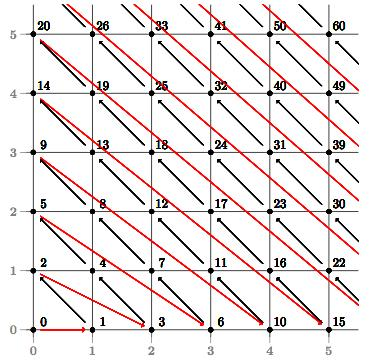
\includegraphics[width=6.5cm,height=4.7cm]{img/cantor-pairing.jpg}
    \caption{Visualization of the Cantor pairing function mapping two-dimensional coordinates to a single value}
    \label{fig:cantor}
\end{figure}

\vspace{5mm}

\section{Space Filling Curves}
Space Filling Curves are mathematical curves that pass through every point in a multi-dimensional space. They provide a way to map multi-dimensional data to a single dimension while preserving spatial locality, making them valuable for spatial indexing and data organization.

The most common space-filling curves include:
\begin{itemize}
    \item \textbf{Z-order Curve}
    \item \textbf{Hilbert Curve}
\end{itemize}

\vspace{5mm}

\begin{figure}[h]
    \centering
    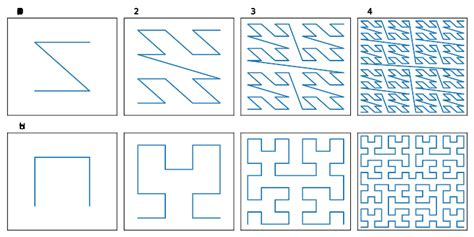
\includegraphics[width=6.5cm,height=4.7cm]{img/hilbert-z-order.jpg}
    \caption{Comparison of Z-order and Hilbert curves in two-dimensional space}
    \label{fig:space-filling}
\end{figure}

\vspace{5mm}

The Hilbert Curve is particularly notable for its ability to preserve locality, meaning that points that are close in multi-dimensional space remain close in the one-dimensional representation.

On the other hand, the Z-order Curve, preserve the order of positions in a grid-like manner, making it suitable for applications requiring efficient spatial queries. Thus, it's possible to reduce the problem of finding matching points into finding the maximum prefix of two bit strings.

\subsection{Z-order Curve}
As mentioned, the Z-order curve is one of the most widely used space-filling curves. It maps multi-dimensional data into a single dimension, similar to the Cantor encoding function. Conversly, it has some some useful properties, when applied to spacial data, such as preserving locality and allowing efficient range queries.

\subsubsection{Z-order Encoding}

The encoding process for Z-order involves interleaving the bits of the coordinates of a point in a multi-dimensional space. For example, given a point with coordinates \( (x, y) \), the Z-order encoding can be represented as:
\[
    Z(x, y) = \sum_{i=0}^{n} (x_i \cdot 2^{2i} + y_i \cdot 2^{2i+1})
\]

Where:
\begin{itemize}
    \item \( x_i \) and \( y_i \) are the bits of the binary representation of the coordinates \( x \) and \( y \).
    \item \( n \) is the number of bits used to represent each coordinate.
\end{itemize}

\subsubsection{Z-order Decoding}
The decoding process retrieves the original coordinates from the Z-order encoded value. Given a Z-order value \( Z \), the decoding can be performed by extracting the bits corresponding to each coordinate:
\[
    x = \sum_{i=0}^{n} (Z \pmod{ 2^{2i+2} }) \cdot 2^i
\]
Where:
\begin{itemize}
    \item \( Z \pmod{ 2^{2i+2} } \) extracts the bits corresponding to the \( i \)-th coordinate.
    \item The result is then shifted and combined to reconstruct the original coordinate \( x \).
\end{itemize}

\subsubsection{Z-order Querying}
Let's consider a scenario where we want to find all points within a specific range in a two-dimensional space. We define \( P \) as the set of points in the space, and we want to find all points \( p \in P \) such that:
\[
    p.x \in [x_{min}, x_{max}] \quad \text{and} \quad p.y \in [y_{min}, y_{max}]
\]

We can leverage the Z-order encoding to efficiently query this range. This is possible by calculating the order of the encoding that we want to find. 
By definition we can represent the GPS coordinates of a point \( (x_p, y_p) \) into a point \( e_p \). This point will be represented in the space of \( n \) orders, each contained in \( \mathbb{Z}_4 \).

\subsubsection{Maximum Common Prefix Search}
A key operation in Z-order based spatial queries is finding the maximum common prefix between two Z-order encoded values. This operation is fundamental for determinating spatial relationships between points.

Given two Z-order encoded values \( Z_1 \) and \( Z_2 \), we can find the maximum common prefix by following three steps. Firstly, we convert both values to their binary representation. Then, we compare the bits from left to right, stopping at the first position where the bits differ. Finally, we extract the common prefix up to that point. The cited algorithm shows that in the worst case, the maximum common prefix can be found in \( O(n) \) time, where \( n \) is the number of bits in the Z-order encoding.

The length of the common prefix determines the size of the smallest bounding box that contains both points. This property is particularly useful for:
\begin{itemize}
    \item Finding the smallest region containing multiple points
    \item Determining if points are within a certain distance of each other
    \item Optimizing spatial range queries
\end{itemize}

For example, consider two points with Z-order encodings:
\begin{align*}
    Z_1 &= 3310_4 \\
    Z_2 &= 3312_4
\end{align*}
The maximum common prefix is \( 331_4 \), indicating that these points share the same region in the first three orders of the encoded space. We used base 4 because it's the easiest way to visualize which of the four quadrants the point belongs to, as each digit represents a quadrant in a two-dimensional space.

This prefix-based approach can be extended to handle range queries by:
\begin{enumerate}
    \item Encoding the query range boundaries
    \item Finding the maximum common prefix of the range
    \item Generating all possible Z-order values that share this prefix
\end{enumerate}

The efficiency of this approach comes from the fact that we can perform these operations using simple bitwise operations, making it suitable for real-time applications.


\section{Privacy Preserving}
Privacy Preserving techniques ensure the protection of sensitive information while allowing necessary computations and data processing. These methods are crucial in maintaining confidentiality in distributed systems and data analysis. For example, in the context of location-based services, privacy-preserving techniques allow for the sharing of location data without revealing exact coordinates, thus protecting user privacy.

\subsection{Homomorphic Encryption}
Homomorphic Encryption(HE) is a form of encryption that allows specific types of computations to be performed on ciphertext, producing an encrypted result that, when decrypted, matches the result of operations performed on the plaintext.

Let's denote \( \xi_k \) as the encryption function, \( \xi_k^{-1} \) as the decryption function, and \( f \) as a function that can be computed on plaintexts. Homomorphic Encryption satisfies the property:
\[
    \xi_k(f(x)) = f(\xi_k(x))
\]

\subsubsection{Fully Homomorphic Encryption}
Fully Homomorphic Encryption (FHE) enables arbitrary computations on encrypted data without decryption. It allows for complex operations while maintaining data privacy, although it comes with significant computational overhead.

\subsubsection{Partially Homomorphic Encryption}
Partially Homomorphic Encryption (PHE) supports only specific types of operations (like addition or multiplication) on encrypted data. While more limited than FHE, it offers better performance and is feasible for applications requiring specific mathematical operations.

\section{Usage of HE for Matching}
Homomorphic Encryption can be used to securely match location. To archive this, we can use different techniques such as:
\begin{itemize}
    \item \textbf{Distance Calculation}: It is archived by tweeking the distance calculation algorithms (e.g., Euclidean distance, Cosine similarity, Manhattan Distance) to work with encrypted coordinates. The main limit comes with the constraint that the operations must be compatible with the encryption scheme used. For instance, calculating the squared Euclidean distance between two points \( (x_1, y_1) \) and \( (x_2, y_2) \) can be expressed as:
    \[
        d^2 = (x_1 - x_2)^2 + (y_1 - y_2)^2
    \]
    That can be computed homomorphically, and then decrypted before computing the square root to get the actual distance.
    \item \textbf{Encoding Coordinates}: By encoding coordinates into a grid-like structure, we can reduce the problem into finding two different points sharing the same area-encoding. This apporach comes with some limitations, mainly related to the precision of the approximation and the size of the grid. Still, it allows for efficient matching of points within a specific area without revealing their exact coordinates.
\end{itemize}

\subsubsection{Privacy-Preserving Z-order Queries}
When implementing privacy-preserving location queries using Z-order encoding, we can employ homomorphic encryption to protect sensitive location data \cite{zhang2020privacy}. Let's consider a scenario where a user \( A \) wants to share their location with user \( B \) while maintaining privacy:

\begin{itemize}
    \item Let \( QK_A \) be the QuadKey representation of \( A \)'s location
    \item Let \( M_B \) be the bit mask specified by \( A \) for user \( B \)
    \item The service provider (SP) performs homomorphic multiplication: \( QK_A \otimes M_B \)
\end{itemize}

To ensure unambiguous results, we increment each value in \( qk_i \in QK_A \) by one before encryption, such that \( qk_i \in \{1,2,3,4\} \). In this scheme \cite{zhang2020privacy}:
\begin{itemize}
    \item A bit mask value of 1 preserves the location data
    \item A bit mask value of 0 masks the location data
\end{itemize}

After decryption on the client device, we:
\begin{enumerate}
    \item Remove any zero values
    \item Convert the elements back to \( \mathbb{Z}_4 \)
    \item Generate a masked QuadKey string that produces a bounding box with the desired level of detail
\end{enumerate}

This approach is computationally efficient as it requires only one round of homomorphic multiplication. The resulting bounding box effectively hides both precise locations and movement patterns, providing privacy even against colluding users.

For example, given a precise GPS coordinate \( (43.084451, -77.680069) \), the system can generate bounding boxes of varying sizes based on the privacy preferences (where \( d \) represents the level of detail). This ensures that location data is shared at an appropriate granularity while maintaining user privacy.

\subsection{PHE and FHE Implications}
The choice between Partially and Fully Homomorphic Encryption has significant implications for system performance, security, and functionality. As previously discussed, the two methods used for proximity checks in a location-based scenario require careful consideration of the encryption scheme.

If the requirements only involve checking whether two positions share a common area, leveraging the speed and simplicity of the Z-order approach is recommended. Conversely, if the goal is to compute a precise floating-point distance value, a homomorphically encrypted distance function (e.g., Euclidean distance) may be necessary. However, it is important to note that in this case, the final result may be affected by computational noise inherent to FHE operations.

\chapter{System Architecture}
In this chapter, we present the system arhcitecture for the proposed privacy-preserving location matching protocol. The main idea is to apply the principles of homomorphic encryption to location-based services, allowing clients to securely publish and query their positions without revealing sensitive information.

\section{Study case}
To deeply understand the system operations, let's first analyze the use case of a client that wants to find the closest parking spot available. The client needs to obtain the position from the sensors, compute the distances between its position and the parking spots, and finally decide whether to park or not.

Even through it seems a simple and straightforward mechanism, if we want to move the operations to the server, in order to preserve computational resources on the client side, a lot of challenges aries. The first one is to securely share the position of the client with the server, without exposing it to the workers. The second challenge is to compute the distances between the positions of the clients and the parking spots, without revealing the positions of the clients to the workers. The third problem is not to leak sensible information about the clients, after the computation is finished.

In this scenario, it's not enough to simply encrypt the positions of the clients, as the workers need to compute the distances between the positions of the clients and the parking spots, that are also encrypted with a different key. To resolve this problem, we could just leave the parking position cleartext on the database, but this would expose the parking spots to the workers, that could then leak the information for profit. In order to avoid this, and also achieve a full zero-knowledge protocol, we need to use a re-encryption mechanism, that allows the workers to compute the distances between the positions of the clients and the parking spots, without revealing the positions of the clients to the workers.

The distance problem is avoided by using the Z-order encoding, that allows us to reduce the problem of finding matching points into finding the maximum prefix of two bit strings. In our showcase, the simulated server will perform a simple encrypted subtraction between the positions of the clients and the parking spots to reveal if the two point are the same or not by checking if the result is zero. 

\section{System Overview}
The protocoll is designed to compbine a standard request-response protocol with a publish-subscribe mechanism.


\begin{figure}[h]
    \centering
    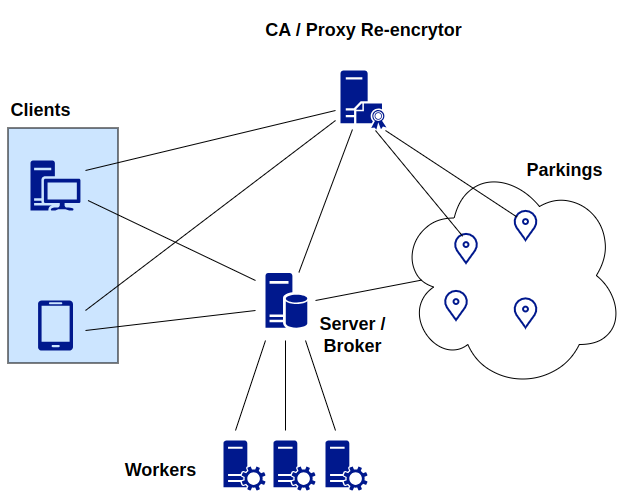
\includegraphics[width=8.5cm,height=5.5cm]{img/architecture-scheme.png}
    \caption{Visualization of the system architecture for the proposed privacy-preserving location matching protocol.}
    \label{fig:architecture}
\end{figure}

Homomorphic encryption incurs high computational costs, so the system optimizes performance by splitting the workload: the server handles only essential data processing, while workers compute the distances between client positions. Since HE allows computations on encrypted data, this approach preserves the privacy of clients' locations without compromising efficiency.

\section{Actors}

\subsection{LDS}
The Location Data Source (LDS), commonly referred to as sensors or parkings, are responsible for collecting and publishing location data. In our system, we assume they indipendently publish their data to the broker, based on the event they register. For instance, if a sensor detects a free parking spot, it publishes the information to the broker, that will start the encryption protocol. This appens also when a parking spot is occupied, allowing the system to keep track of the available parking spots in real-time.

Note that by maintaining the availability of the parking spots, independent from the clients, we can ensure that the system is able to provide privacy-preserving updates to the server. Conversely, if the clients were also responsible for reserving the parking spots, they would need to expose their positions to the server, which would compromise the privacy of the system.

\subsection{MC}
MCs or Mobile Clients are the users of the system. Their main interest is to receive updates on the closest available parking spots, based on their current position. 

In our system, the clients responsibilies are very limited, as they do not trust the server and all the other actors involved in the protocol. They only need to publish their position to the server, wait for the computation to finish, and then receive the results.

\subsection{Server}
The Backend Server (commonly called Information Broker) is the central component of the system, responsible for managing the communication between clients and sensors. It also acts like a database, handling and storing the encrypted parking spots data.

This centralized component is crucial in the architecture, as it allows all sort of mobile actors (including clients and LDs) to have a persistent connection with the system, altough it's not enough if we want to achieve a full zero-knowledge protocol.

\subsection{Proxy}
The Proxy (Re-encryptor) is an intermediary component that facilitate the connection between clients and the server.

It utilize the MQTT protocol to manage the comunication with the client. Moreover, it keeps alive the TCP connection with the client (that usually has a natted IP address) and the broker.
This is accomplished by making the client subscribe to the connection topic, while the proxy publishes the updates to the server about the client requests.

This approach allows the user to have a persistent connection, without the need to maintain a direct TCP connection with the server. The proxy is also responsible for managing the re-encryption of the data, ensuring that the server (and the workers) can compute the calculations on ciphertext encrypted with the right keys.

\subsection{Worker}
The name Worker refers to a generic computational unit of the system, that can handle tasks from the server, rewarded with a digital currency. In our case, the workers are responsible for computing the distances between the positions of the clients and the parking spots, using the homomorphic encryption scheme. 

The workers's digial reward can be described as a token, that allows them to request tasks from the server. In this way, each client can act as a worker, contributing to the overall computation of the system.

\section{Network Protocol and Communication}
\subsection{MQTT}

The MQTT protocol is used for the communication between the clients and the proxy. It's necesassry to use a pub/sub mechanism in order to keep alive the connection between the two entities. This is achived by having the client subscribe to a topic, while the proxy publishes updates to that topic.

Moreover, the proxy is responsible for managing the connection with the broker, allowing the clients to receive updates on the parking spots without exposing their positions. In this way, the client $MC_i$ \textbf{publishes} its position $Area_j$ to the topic $ID_{MC_i}$. The proxy then forwards the position to the broker, which stores the encrypted positions of the parking spots.

When the computation is finished, the broker publishes the results to the topic $ID_{MC_i}$, allowing the client to receive the updates on the parking spots. The client can then \textbf{subscribe} to the topic $ID_{MC_i}$ to receive updates on the parking spots.

\subsection{HTTP}
The HTTP protocol is used for all the traffic arriving and leaving the backend server. The server is responsible for managin the storage of the encrypted parking spots data, for handling the requests from the proxy(s) and managing the workers.

Beacause the backend server acts also as a database, it is responsible for storing the encrypted positions of the parking spots, and for managing the requests from the clients. Thus, it provides an HTTP API for the clients to interact with the system. 

%\newpage

\section{Protocol Overview}
The system is designed to allow the following operations:

\begin{table}[h]
%\setlength\tabcolsep{3pt}
\renewcommand{\arraystretch}{1.3}
\small
%\begin{tabularx}{\linewidth}{|l|p{1.6cm}|p{2cm}|p{2cm}|p{4cm}|}
\begin{tabularx}{\linewidth}{|l|X|X|X|p{4cm}|}
\hline
\textbf{API} & \textbf{Subject} & \textbf{Protocol} & \textbf{Receiver} & \textbf{Payload} \\ \hline
Position Publish & MC & MQTT Sub & Proxy & $\{position: \xi_{mc}( P_i )\}$ \\ \hline
Key Obtain & MC & HTTP GET & Backend & - \\ \hline
Key publish & MC & HTTP POST & Proxy & $\{keys: \newline [\forall j \in \text{P},\ k_{mc_i, park_j}]\}$ \\ \hline
Parking Request & Proxy & MQTT Pub & Backend &
$\{proxy: p_i,\ positions: \newline [\forall j \in \text{P},\ \xi_{mc_i, park_j}(P_i)]\}$ \\ \hline
Parking Publish & LDS & POST & Backend & $\{\xi_{park_j}(P_j), k_{park_j}^+\newline \text{status} \in \{\text{free}, \text{occ.}\}\}$ \\ \hline
Work Request & Worker & HTTP POST & Backend & - \\ \hline
Task Finish & Worker & HTTP POST & Backend & $\{worker: w_i,\ task: t_j,\newline result: \xi_{mc_i, park_j}(R)\}$ \\ \hline
Computation Resoult & Backend & MQTT Pub & Proxy & $\{proxy: p_i,\ resoult: \newline [\forall j \in \text{P},\ \xi_{mc_i, park_j}(R)]\}$ \\ \hline
Distances Publish & Proxy & MQTT Pub & MC & $\{distances: [\forall j \in \text{P},\ \xi_{mc_i}(R)]\}$ \\ \hline
\end{tabularx}
\caption{The System Operations}
\label{table:system-operations}
\end{table}

\newpage
\section{Scenario}
\begin{figure}[h]
    \centering
    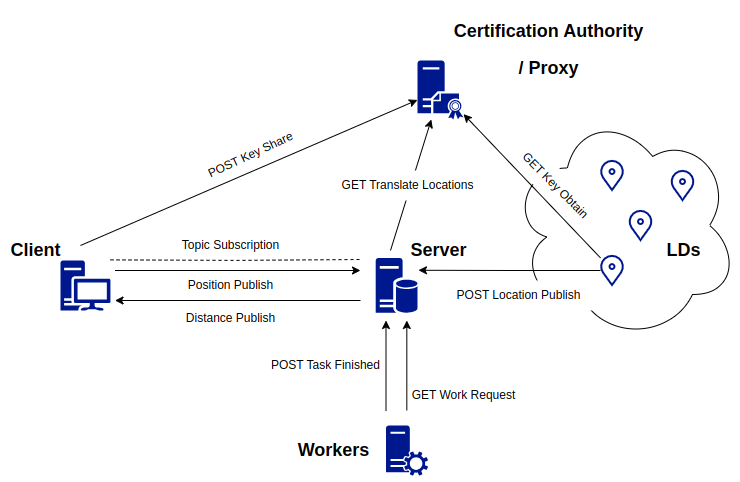
\includegraphics[width=12cm,height=7.5cm]{img/workflow.png}
    \caption{Visualization of the protocol flow}
    \label{fig:protocol-flow}
\end{figure}

We can summarize the protocol flow in the following steps:

\subsection{Protocol Flow}
\begin{enumerate}
    \item The mobile client $MC_i$ initiates a public-keys retrieval by invoking the \textbf{Key Obtain} API via an HTTP GET request to the backend server. \emph{(API: \texttt{Key Obtain}, Payload: none) \to Keys: $[\forall p_j \in P, \xi_{p_j^+}]$)}
    \item For each parking spot $park_j$, the client $MC_i$ generates a symmetric translation key $k_{mc_i, park_j}$ and sends the collection to the proxy using the \textbf{Key Publish} API via an HTTP POST request. \emph{(API: \texttt{Key Publish}, Payload: $\{keys: [\forall j \in \text{P},\ k_{mc_i, park_j}]\}$)}
    \item The client $MC_i$ then publishes its encrypted position $\xi_{mc}(P_i)$ to the MQTT topic $ID_{MC_i}$ using the \textbf{Position Publish} API. \emph{(API: \texttt{Position Publish}, Payload: $\{position: \xi_{mc}(P_i)\}$)}
    \item The proxy subscribes to the topic, receives the encrypted position, and re-encrypts it for each parking spot using the associated key $k_{mc_i, park_j}$, creating the re-encrypted blob $[\forall j \in \text{P},\ \xi_{mc_i, park_j}(P_i)]$. It then invokes the \textbf{Parking Request} API via MQTT to publish this to the backend. \emph{(API: \texttt{Parking Request}, Payload: $\{proxy: p_i,\ positions: [\ldots]\}$)}
    \item Each local data source (LDS) publishes its own position $\xi_{park_j}(P_j)$ and occupancy status via the \textbf{Parking Publish} API using an HTTP POST request to the backend. \emph{(API: \texttt{Parking Publish}, Payload: $\{\xi_{park_j}(P_j),\ status\}$)}
    \item The backend, upon receiving new position updates, issues a \textbf{Work Request} to available workers via HTTP POST, initiating the task computation. \emph{(API: \texttt{Work Request}, Payload: none)}
    \item Once the workers compute the distances (or other metrics) between client and parking spots, they send the result back using the \textbf{Task Finish} API. \emph{(API: \texttt{Task Finish}, Payload: $\{worker: w_i,\ task: t_j,\ result: \xi_{mc_i, park_j}(R)\}$)}
    \item The backend then publishes the aggregated results to the proxy via MQTT using the \textbf{Computation Resoult} API. \emph{(API: \texttt{Computation Resoult}, Payload: $\{proxy: p_i,\ resoult: [\ldots]\}$)}
    \item Finally, the proxy receives the re-encrypted results, decrypts them using the shared keys, and delivers them to the mobile client $MC_i$.
\end{enumerate}

\section{Security Considerations}

The main goal of the study is to provide a privacy-preserving location matching protocol, that allows clients to securely publish and query their positions without revealing sensitive information. In order to fulfill this goal, we need to ensure that the system is attack-resistant and that the privacy of the clients is preserved.

In the previous implementation\cite{genova2024helamqtt}, the logic behind the position matching protocol relied on the evaluation of the euclidian distance between the positions of the clients and the parking spots from a trusted CA. This approach, even tought hided from the server the raw positions of the clients, leaked information of the MC. This was accomplished by allowing an attacker to perform a \emph{binary search} of the client position, by sending a series of location requests based on the topics the clients subscribed to. By narrowing down the search space, the attacker could eventually find the exact position of the client, thus compromising its privacy.

This showcased that HE is secure if and only if the encryption & decryption operation are performed correctly, preferably by the client itself.

Another really serious isssue with the Genova's protocol is that that there's no way to ensure that the user is really itself. Moreover, if an attacker is able to read the network traffic, he could easily impersonate the client and send fake position updates to the server, or even worse, apply the previous described attack.

In my own implementation, I addressed those issues by introducing different techniques from the state of the art, such as using a proxy re-encryptor and a position encoding mechanism based on Z-order. The choice of leaving the the decryption operation to the client ensures that no one is able to read the sensitive data, despite an increase of computational resources required to re-encrypt each position for each parking spot.

\chapter{Testing}
\section{Testing Methodology}

\section{Performance Evaluation}

\section{Security Analysis}

\chapter{Project}
\section{Glossary}
\begin{itemize}
    \item LDS: Sensors
    \item MC: Clients
\end{itemize}

\section{Project Idea}
L'idea centrale consiste nell'applicare i principi della \emph{homomorphic encryption} al protocollo \emph{LA-MQTT}. Quando un client invia un aggiornamento di posizione, questa viene trasmessa in forma cifrata mediante Fully Homomorphic Encryption (FHE). Il server esegue un'analisi sulle posizioni disponibili, appartenenti alla stessa area geografica, e dopo aver effettuato un controllo con la chiave di verifica, restituisce un blob cifrato contenente le distanze calcolate.

\subsection{Funzionalità Principali}
\begin{itemize}
    \item \textbf{Position Publish}: Il client aggiorna la propria posizione per ricevere informazioni dai publisher relativamente ai sensori presenti nell'area di interesse.
    \begin{itemize}
        \item $Enc(GPS\_DATA)$
        \item $P_{i}$: Posizione
    \end{itemize}
    
    \item \textbf{Area Subscription}: Un client si sottoscrive a un'area di interesse. Per ogni aggiornamento di posizione viene effettuato un controllo su tutte le posizioni riportate fino a quel momento appartenenti all'area.
    \begin{itemize}
        \item $C(i, t_{s})$
    \end{itemize}
    
    \item \textbf{Geofence Publish}: Permette ai client LDS di pubblicare un blob contenente:
    \begin{itemize}
        \item Dati geofence (formato GEOJSON RFC 7946)
        \item $g_s$: geofence target
        \item $c_{s}$: contenuto pubblicizzato
        \item $t_{s}$: topic
        \item $e_{s}$: evento di mobilità
    \end{itemize}
\end{itemize}

\section{Attori del Sistema}
\begin{itemize}
    \item \textbf{Broker/Proxy}: Gestisce le chiavi di tutti i client che hanno effettuato almeno una sottoscrizione
    \item \textbf{Publisher}: Pubblicano aggiornamenti sulle posizioni disponibili
    \item \textbf{Subscriber}: Sottoscrivono aree geografiche e ricevono aggiornamenti sui parcheggi disponibili
\end{itemize}

\section{Vantaggi}
\begin{itemize}
    \item Dati sempre cifrati
    \item In caso di \emph{re-encryption}, solo il proxy conosce le posizioni decifrate dei sensori
    \begin{itemize}
        \item Un proxy malevolo non compromette la posizione dell'utente
        \item Possibile individuare proxy fittizi mediante falsi aggiornamenti di posizione
    \end{itemize}
\end{itemize}

\section{Svantaggi}
\begin{itemize}
    \item Latenze significative (worker)
    \item Attenzione necessaria alla triangolazione delle posizioni
\end{itemize}

\section{Stack Tecnologico}
\begin{itemize}
    \item \textbf{Soluzione ad alte prestazioni}:
    \begin{itemize}
        \item C++ SEAL (Microsoft)
        \item Rust TFHE-rs (ZAMA)
    \end{itemize}
    \item \textbf{Proof of Concept}:
    \begin{itemize}
        \item Python Concrete (ZAMA)
    \end{itemize}
\end{itemize}

\section{Interrogativi Aperti}
\begin{itemize}
    \item \textbf{Prestazioni}: È accettabile un delay di 5-10 secondi per l'analisi dei dati?
    \item \textbf{Re-encryption}: È una soluzione eccessiva?
    \begin{itemize}
        \item Il server salva le posizioni cifrate nel database
        \item Possibile alternativa: Private Set Intersection (PSI)
    \end{itemize}
    \item \textbf{Architettura}: Request-Response vs MQTT
\end{itemize}

\section{Sviluppi Futuri}
\begin{itemize}
    \item Integrazione della libreria \emph{SEAL Embedded} per i sensori
    \item Definizione della funzione per il calcolo delle distanze
    \item Analisi degli ordini di grandezza degli errori
    \item Selezione delle posizioni rilevanti:
    \begin{itemize}
        \item Area poligonale (due punti)
        \item Area discreta (MGRS)
    \end{itemize}
    \item Deduplicazione di vettori numerici
    \item Ottimizzazione delle richieste per evitare attacchi DoS
    \begin{itemize}
        \item Dimostrazione delle vulnerabilità nell'implementazione precedente
        \item Proposta di patch risolutive
    \end{itemize}
\end{itemize}


\section{riferimenti}
Come detto prima le label servono per riferirsi ad altre parti del testo citate precendentemente.\\
Ti consiglio di metterle sempre almeno a figure. immagini e capitoli.

Per riferirti a qualcosa basta fare ref seguito dal nome della label, ad esempio ``vedi capitolo \ref{chap:intro}''.\\In questo modo dal pdf cliccando sulla reference, ti porta direttamente al punto giusto.
Altri pacchetti come \texttt{fancyref} e \texttt{cleveref} (consigliato) possono aiutare nell'automatizzare la creazione delle refrence. Usando ad esempio \texttt{\cref{chap:intro}} viene generata la dicitura corrispondete all'elemento a cui si fa riferimento, seguita dalla numerazione. Eccone un esempio: \cref{chap:intro}.
\section{citazioni}

Se non ti piace lo stile di citazione puoi modificarlo sopra dove scrivo usepackage natbib, ma quello impostato attualmente dovrebbe andare bene.



\renewcommand{\bibsection}{}
\chapter*{References}
\bibliography{refs}
\newpage

\renewcommand{\appendixtocname}{Appendices}
% \csname @openrightfalse\endcsname
\pagenumbering{gobble}

\newpage~\newpage
\chapter*{Ringraziamenti}
Grazie a tutti
\end{document}
